\documentclass[a4paper,12pt]{report}
\usepackage[utf8]{inputenc}
\usepackage{lmodern}
\usepackage{enumitem}
\usepackage{titlesec}
\usepackage{graphicx}
\usepackage{tabularx}
\usepackage{amsmath}
\usepackage{amssymb}
\usepackage[italian]{babel}
\usepackage[margin=2cm]{geometry}

\title{Progetto 20050704 (P.20050704) - RainAir}
\author{Sebastiano Deodati}

\titleformat{\chapter}[display]{\normalfont\huge\bfseries}{}{0pt}{\Huge}

\begin{document}
  \maketitle
  \tableofcontents

  \chapter{Dati di interesse e funzionalità richieste}
    \begin{enumerate}[label=\arabic*.]
      \item clienti
      \begin{enumerate}[label*=\arabic*.]
          \item nome
          \item cognome
          \item indirizzo (req. 8)
          \item frequent flyers
          \begin{enumerate}[label*=\arabic*.]
              \item codice
              \item data di affiliazione
              \item miglia accumulate
          \end{enumerate}
      \end{enumerate}
      \item voli
      \begin{enumerate}[label*=\arabic*.]
          \item codice
          \item miglia percorse
          \item orario e aeroporto di partenza (req. 4)
          \item orario e aeroporto di arrivo (req. 4)
          \item velivolo (req. 5)
      \end{enumerate}
      \item prenotazioni
      \begin{enumerate}[label*=\arabic*.]
          \item prenotante (req. 1)
          \item istante
          \item biglietti (req. 6)
          \item posti
          \item data
          \item eventuale hotel (req. 7) con date di check-in e check-out e stanze prenotate
      \end{enumerate}
      \item aeroporti
      \begin{enumerate}[label*=\arabic*.]
          \item codice
          \item nome
          \item città (req. 9)
          \item tassa di decollo
          \item tassa di atterraggio
      \end{enumerate}

      \newpage

      \item velivoli
      \begin{enumerate}[label*=\arabic*.]
          \item codice
          \item tipo
          \item posti
          \item costo/miglio
      \end{enumerate}
      \item bliglietti
      \begin{enumerate}[label*=\arabic*.]
          \item volo
          \item prezzo base, calcolato sulla base dei costi che la compagnia deve sostenere \\
            ($\frac{[miglia\;effettuate]*[costo/miglio\;del\;velivolo] + [tasse\;di\;decollo\;e\;atterraggio]}{[posti\;del\;velivolo]} * 1,2$)
      \end{enumerate}
      \item hotel
      \begin{enumerate}[label*=\arabic*.]
          \item nome
          \item indirizzo (req. 8)
          \item categoria (da 1 a 5)
          \item tariffa stanza per notte
          \item distanza dal centro
          \item aeroporto più vicino (req. 4) con relativa distanza
      \end{enumerate}
      \item Indirizzi
      \begin{enumerate}[label*=\arabic*.]
          \item via/pza
          \item civico
          \item CAP
          \item città (req. 9)
      \end{enumerate}
      \item città
      \begin{enumerate}[label*=\arabic*.]
          \item nome
          \item stato
      \end{enumerate}
      \item funzionalità richieste
      \begin{enumerate}[label*=\arabic*.]
          \item Il Sistema prenotazioni necessita di calcolare il numero di posti disponibili all'istante corrente su un dato volo di una certa data. Il numero di posti disponibili è calcolato a
                partire dal numero di posti del velivolo che effettua il volo in questione, diminuito del numero di posti già prenotati (all’istante corrente).

          \newpage

          \item Il Sistema prenotazioni deve anche poter calcolare il prezzo complessivo, all’istante corrente, di un certo numero di biglietti per un volo di un dato giorno. Tale prezzo è
                da considerarsi valido solo nel caso in cui il volo disponga, al momento corrente, di un numero sufficiente di posti per la data richiesta, e si calcola moltiplicando il prezzo di
                un biglietto singolo per il numero di biglietti richiesti. Il prezzo di un singolo biglietto è altamente flessibile, ed è composto da diverse componenti, dovute a diversi fattori:
                \begin{itemize}
                  \item Il prezzo base, che dipende dal volo
                  \item Il numero di posti disponibili al momento corrente per la data di volo richiesta.
                \end{itemize}
                Il calcolo del prezzo del biglietto parte dal suo prezzo base, e subisce poi delle modifiche a seconda della disponibilità attuale di posti sulla data di volo richiesta.
                In particolare, al prezzo base si applica la seguente regola: se il numero di posti disponibili al momento della prenotazione per il volo in questione è maggiore della metà
                dei posti totali (ovvero quelli del velivolo che effettua il volo), si applica uno sconto del 2\% per ogni posto libero oltre la metà. Al contrario, se il numero di posti
                disponibili è minore della metà, si applica un sovrapprezzo del 2\% in modo del tutto analogo.
          \item Il Sistema prenotazioni vuole offrire anche il seguente servizio: data una città e una tariffa massima, vuole suggerire un insieme di hotel in quella città che abbiano tutti una
                tariffa al più pari a quella indicata. La scelta degli hotel avviene secondo le seguenti regole (a parte quella sulla tariffa, che deve essere sempre rispettata):
                \begin{itemize}
                  \item Farà parte del risultato l’hotel più vicino al centro della città in questione con tariffa entro la soglia; sia questo hotel $A$.
                  \item Farà inoltre parte del risultato qualunque altro hotel con lo stesso numero di stelle di $A$ che abbia una distanza dal centro pari al più il 110\% di quella di $A$.
                  \item Infine, faranno parte del risultato anche quegli hotel che hanno più stelle di $A$, ma più lontani di $A$ dal centro. In particolare, quelli per cui la distanza
                        dal centro sia al massimo il 120\% di quella di $A$.
                \end{itemize}
          \item Il sistema deve inoltre gestire il sistema di benefici dei "frequent flyers", dove il numero di miglia calcolate è dato dalla somma delle miglia per ogni singolo volo moltiplicate
                per il numero di posti della relativa prenotazione, effettuati dopo la data di affiliazione. Queste miglia raddoppiano se la prenotazione include anche un hotel fino a 4 stelle,
                e triplicano se l'hotel è a 5 stelle.
      \end{enumerate}
    \end{enumerate}

  \chapter{Diagramma ER}
    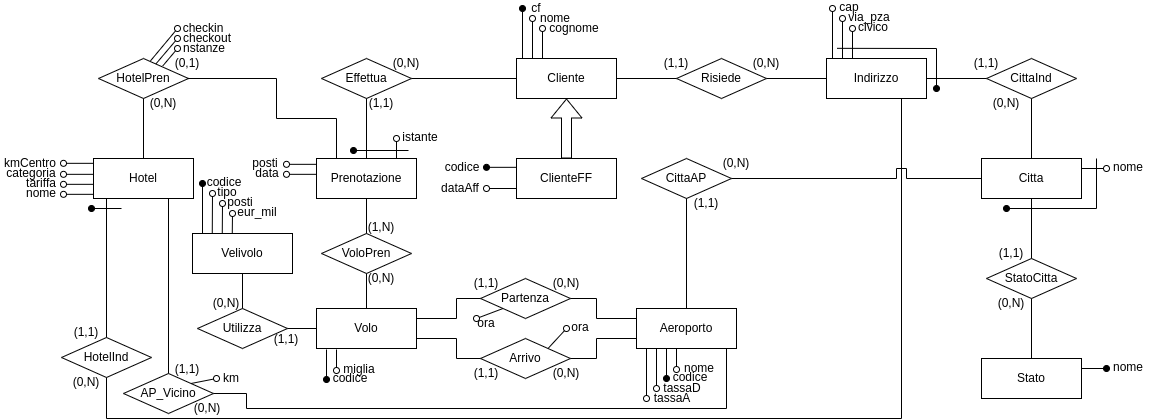
\includegraphics[width=1\textwidth]{er.png}

  \chapter{Dizionario dei dati}
    Entità Cliente: \\
      \begin{tabular}{|c|c|c|}
        \hline Attributo & Tipo & Note \\
        \hline cf & cf & stringa in formato CF \\
        \hline nome & stringa & \\
        \hline cognome & stringa & \\
        \hline
      \end{tabular} \\ \\
    Entità ClienteFF: \\
      \begin{tabular}{|c|c|c|}
        \hline Attributo & Tipo & Note \\
        \hline codice & intero $>$ 0 & \\
        \hline dataAff & data & \\
        \hline
      \end{tabular} \\ \\
      Entità Volo: \\
      \begin{tabular}{|c|c|c|}
        \hline Attributo & Tipo & Note \\
        \hline codice & iata\_fl & codice volo \\
        \hline miglia & intero $>$ 0 & \\
        \hline
      \end{tabular} \\
      V.Volo.part\_arr: $\forall v, p, a, o_p, o_a \; $Volo$(v) \wedge $Partenza$(v, p) \wedge ora(v, p, o_p) \wedge $Arrivo$(v, a) \wedge ora(v, a, o_a) \\
      \hspace*{1cm}\rightarrow\; p \neq a$ \\
      V.Volo.no\_overbooking: $\forall v, d \; $Volo$(v) \wedge $data$(d) \;\rightarrow\; $Posti\_Voli.Posti\_Disponibili$(v, d) \geq 0$ \\ \\
      Entità Prenotazione: \\
      \begin{tabular}{|c|c|c|}
        \hline Attributo & Tipo & Note \\
        \hline istante & dataora & \\
        \hline posti & intero $>$ 0 & \\
        \hline data & data & \\
        \hline
      \end{tabular} \\ \\
      Entità Aeroporto: \\
      \begin{tabular}{|c|c|c|}
        \hline Attributo & Tipo & Note \\
        \hline codice & iata\_ap & codice aeroporto IATA \\
        \hline nome & stringa & \\
        \hline tassaD & valuta $>$ 0 & \\
        \hline tassaA & valuta $>$ 0 & \\
        \hline
      \end{tabular} \\ \\
      Entità Velivolo: \\
      \begin{tabular}{|c|c|c|}
        \hline Attributo & Tipo & Note \\
        \hline codice & plane\_reg & codice di registrazione velivolo \\
        \hline tipo & stringa & \\
        \hline eur\_mil & valuta $>$ 0 & \\
        \hline posti & intero $>$ 0 & \\
        \hline
      \end{tabular} \\ \\

      \newpage

      \hspace*{-0.75cm}
      Entità Hotel: \\
      \begin{tabular}{|c|c|c|}
        \hline Attributo & Tipo & Note \\
        \hline nome & stringa & \\
        \hline categoria & intero [1, 5] & \\
        \hline tariffa & valuta $>$ 0 & \\
        \hline kmCentro & intero $\geq$ 0 & \\
        \hline
      \end{tabular} \\ \\
      Entità Indirizzo: \\
      \begin{tabular}{|c|c|c|}
        \hline Attributo & Tipo & Note \\
        \hline via\_pza & stringa & \\
        \hline civico & intero $\geq$ 0 & 0 indica SNC \\
        \hline cap & stringa CAP & \\
        \hline
      \end{tabular} \\ \\
      Entità Citta: \\
      \begin{tabular}{|c|c|c|}
        \hline Attributo & Tipo & Note \\
        \hline nome & stringa & \\
        \hline
      \end{tabular} \\ \\
      Entità Stato: \\
      \begin{tabular}{|c|c|c|}
        \hline Attributo & Tipo & Note \\
        \hline nome & stringa & \\
        \hline
      \end{tabular} \\ \\
      Relationship HotelPren: \\
      \begin{tabular}{|c|c|c|}
        \hline Attributo & Tipo & Note \\
        \hline checkin & data & \\
        \hline checkout & data & \\
        \hline nstanze & intero $>$ 0 & \\
        \hline
      \end{tabular} \\
      V.HotelPren.checkin\_checkout: $\forall h, p, i, o \; Hotel(h) \wedge HotelPren(h, p) \wedge \\
      \hspace*{1cm}checkin(h, p, i) \wedge checkout(h, p, o) \;\rightarrow\; i \leq o $ \\ \\
      Relationship AP\_Vicino: \\
      \begin{tabular}{|c|c|c|}
        \hline Attributo & Tipo & Note \\
        \hline km & intero $>$ 0 & \\
        \hline
      \end{tabular} \\ \\
      Relationship Partenza: \\
      \begin{tabular}{|c|c|c|}
        \hline Attributo & Tipo & Note \\
        \hline ora & ora & \\
        \hline
      \end{tabular} \\ \\
      Relationship Arrivo: \\
      \begin{tabular}{|c|c|c|}
        \hline Attributo & Tipo & Note \\
        \hline ora & ora & \\
        \hline
      \end{tabular} \\ \\

    \chapter{UML}
      \begin{center}
        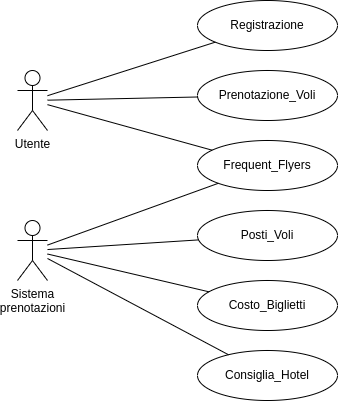
\includegraphics{uml.png}
      \end{center}

    \chapter{Specifiche degli use-case}
      \section{Specifiche use-case Registrazione}
        \hspace*{1cm}Registra(cf: cf, nome: stringa, cognome: stringa, residenza: Indirizzo) : Cliente \\
        \hspace*{2cm}precondizioni: $\neg \exists c Cliente(c) \wedge cf(c, cf)$ \\
        \hspace*{2cm}postcondizioni: \\
        \hspace*{3cm}modifica al livello estensionale dei dati: \\
        \hspace*{4cm}nuovi elementi del dominio di interpretazione: c \\
        \hspace*{4cm}nuove ennuple di predicati: \\
        \hspace*{5cm}Cliente(c) \\
        \hspace*{5cm}cf(c, cf) \\
        \hspace*{5cm}nome(c, nome) \\
        \hspace*{5cm}cognome(c, cognome) \\
        \hspace*{5cm}Risiede(c, residenza) \\
        \hspace*{3cm}valore di ritorno: result = c \\ \\

      \section{Specifiche use-case Prenotazione\_Voli}
        \hspace*{1cm}Prenota(c: Cliente, v: volo, nposti: intero $>$ 0, giorno: data) : Prenotazione \\
        \hspace*{2cm}precondizioni: $"Posti\_Voli".Posti\_Disponibili(v, giorno) \geq nposti$ \\
        \hspace*{2cm}postcondizioni: \\
        \hspace*{3cm}modifica al livello estensionale dei dati: \\
        \hspace*{4cm}nuovi elementi del dominio di interpretazione: p \\
        \hspace*{4cm}nuove ennuple di predicati: \\
        \hspace*{5cm}Prenotazione(p) \\
        \hspace*{5cm}istante(p, \textit{adesso}) \\
        \hspace*{5cm}posti(p, nposti) \\
        \hspace*{5cm}data(p, giorno) \\
        \hspace*{5cm}Effettua(c, p) \\
        \hspace*{5cm}VoloPren(v, p) \\
        \hspace*{3cm}valore di ritorno: result = p \\ \\

        \newpage

        \hspace*{1cm}Annulla\_Pren(p: Prenotazione) \\
        \hspace*{2cm}precondizioni: $\exists d \text{data}(p, d) \wedge d < \textit{oggi}$ \\
        \hspace*{2cm}postcondizioni: \\
        \hspace*{3cm}modifica al livello estensionale dei dati: \\
        \hspace*{4cm}elementi del dominio di interpretazione che non esistono più: p \\
        \hspace*{4cm}ennuple di predicati non più valide: \\
        \hspace*{5cm}Prenotazione(p) \\
        \hspace*{3cm}valore di ritorno: nessuno \\ \\

        \section{Specifiche use-case Frequent\_Flyers}
        \hspace*{1cm}Affilia(c: Cliente, cod: intero $>$ 0) : ClienteFF \\
        \hspace*{2cm}precondizioni: $\neg ClienteFF(c)$ \\
        \hspace*{2cm}postcondizioni: \\
        \hspace*{3cm}modifica al livello estensionale dei dati: \\
        \hspace*{4cm}dominio di interpretazione: invariato \\
        \hspace*{4cm}nuove ennuple di predicati: \\
        \hspace*{5cm}ClienteFF(c) \\
        \hspace*{5cm}codice(c, cod) \\
        \hspace*{5cm}dataAff(c, \textit{oggi}) \\
        \hspace*{3cm}valore di ritorno: result = c \\ \\

        \hspace*{-0.6cm}
        \hspace*{1cm}Miglia(c: ClienteFF) : intero $\geq$ 0 \\
        \hspace*{2cm}precondizioni: nessuna \\
        \hspace*{2cm}postcondizioni: \\
        \hspace*{3cm}modifica al livello estensionale dei dati: nessuna \\
        \hspace*{3cm}valore di ritorno: \\
        \hspace*{4cm}Sia $P = \{(p, n) | Prenotazione(p) \wedge Effettua(c, p) \wedge posti(p, n) \\
        \hspace*{5cm}\wedge [\exists d,d_a \text{ ata}(p, d) \wedge dataAff(c, d_a) \wedge d \geq d_a]\}$ \\
        \hspace*{4cm}Sia $P_h = \{(p, n) \in P | \exists h \text{HotelPren}(h, p)\}$ \\
        \hspace*{4cm}Siano $P_5 = \{(p, n) \in P_h | \exists h \text{HotelPren}(h, p) \wedge \text{categoria}(h, 5)\}$, \\
        \hspace*{5cm}$P_4 = P_h \setminus P_5$ e $P_{nh} = P \setminus P_h$ \\
        \hspace*{4cm}Sia $V_{nh} = \{(v, m, p, n) | \text{Volo}(v) \wedge \text{miglia}(v, m) \wedge (p, n) \in P \wedge \text{VoloPren}(v, p)]\}$ \\
        \hspace*{4cm}Sia $V_4 = \{(v, m, p, n) | \text{Volo}(v) \wedge \text{miglia}(v, m) \wedge (p, n) \in P_4 \wedge \text{VoloPren}(v, p)]\}$ \\
        \hspace*{4cm}Sia $V_5 = \{(v, m, p, n) | \text{Volo}(v) \wedge \text{miglia}(v, m) \wedge (p, n) \in P_5 \wedge \text{VoloPren}(v, p)]\}$ \\
        \hspace*{4cm}result = $\left(\sum_{(v, m, p, n) \in V_{nh}} m*n\right) + 2*\left(\sum_{(v, m, p, n) \in V_4} m*n\right) + 3*\left(\sum_{(v, m, p, n) \in V_5} m*n\right)$ \\ \\

      \newpage

      \section{Specifiche use-case Posti\_Voli}
        \hspace*{1cm}Posti\_Disponibili(v: Volo, d: data) : intero $\geq$ 0 \\
        \hspace*{2cm}precondizioni: nessuna \\
        \hspace*{2cm}postcondizioni: \\
        \hspace*{3cm}modifica al livello estensionale dei dati: nessuna \\
        \hspace*{3cm}valore di ritorno: \\
        \hspace*{4cm}Sia $P = \{(p, n) | Prenotazione(p) \wedge VoloPren(v, p) \wedge posti(p, n)\}$ \\
        \hspace*{4cm}Sia $a | Velivolo(a) \wedge Utilizza(v, a)$ e sia $max | "intero > 0"(max) \wedge posti(a, max)$ \\
        \hspace*{4cm}result = $max - \sum_{(p, n) \in P} n$ \\ \\

      \section{Specifiche use-case Costo\_Biglietti}
        \hspace*{1cm}Costo(v: Volo, d: data) : valuta $>$ 0 \\
        \hspace*{2cm}precondizioni: nessuna \\
        \hspace*{2cm}postcondizioni: \\
        \hspace*{3cm}modifica al livello estensionale dei dati: nessuna \\
        \hspace*{3cm}valore di ritorno: \\
        \hspace*{4cm}Siano $A_d | \text{Partenza}(v, A_d)$ e $A_a | \text{Arrivo}(v, A_a)$ \\
        \hspace*{4cm}Siano $t_d | "valuta > 0"(t_d) \wedge \text{tassaD}(A_d, t_d)$ e $t_a | "valuta > 0"(t_a) \wedge \text{tassaA}(A_a, t_a)$ \\
        \hspace*{4cm}Siano $mil | "intero > 0"(mil) \wedge \text{miglia}(v, mil)$, \\
        \hspace*{5cm}$eur\_mil | "intero > 0"(eur\_mil) \wedge eur\_mil(v, eur\_mil)$ \\
        \hspace*{4cm}Siano $A | \text{Velivolo}(A) \wedge \text{Utilizza}(v, A)$ e $posti | "intero > 0"(posti) \wedge \text{posti}(A, posti)$ \\
        \hspace*{4cm}Sia $base = \left(\frac{mil \times eur\_mil + t_d + t_a}{posti}\right) \times 1.2$ \\
        \hspace*{4cm}Sia $disp = "Posti\_Voli".\text{Posti\_Disponibili}(v, d)$ \\
        \hspace*{4cm}Sia $disp\_coeff = I(disp \geq posti/2) \times 0.8 \times disp + \\
        \hspace*{5cm}+ I(disp < posti/2) \times 1.2 \times disp$ \\
        \hspace*{4cm}result = $base \times disp\_coeff$ \\ \\

      \section{Specifiche use-case Consiglia\_Hotel}
        \hspace*{1cm}Consiglia\_Hotel(c: Citta, max: valuta $>$ 0) : Hotel(1,N) \\
        \hspace*{2cm}precondizioni: $\exists h, i \text{ Hotel}(h) \wedge \text{HotelInd}(h, i) \wedge \text{CittaInd}(c, i)$ \\
        \hspace*{2cm}postcondizioni: \\
        \hspace*{3cm}modifica al livello estensionale dei dati: nessuna \\
        \hspace*{3cm}valore di ritorno: \\
        \hspace*{4cm}Sia $H = \{(h, t, d, cat) | \text{Hotel}(h) \wedge \text{tariffa}(h, t) \wedge \text{kmCentro}(h, d) \wedge$ \\
        \hspace*{4.5cm}$\text{categoria}(h, cat) \wedge t \leq max \wedge [\exists i \text{ HotelInd}(h, i) \wedge \text{CittaInd}(c, i)]\}$ \\
        \hspace*{4cm}Sia $(A, t_A, d_A, cat_A) \in H | \neg \exists (h, t, d, cat) \in H [d < d_A]$ \\
        \hspace*{4cm}Sia $h_{same} = \{(h, t, d, cat) \text{ in } H | cat = cat_A \wedge d \leq d_A \times 1.1\}$ \\
        \hspace*{4cm}Sia $h_{better} = \{(h, t, d, cat) \text{ in } H | cat > cat_A \wedge d \leq d_A \times 1.2\}$ \\
        \hspace*{4cm}result = $\{A\} \cup h_{same} \cup h_{better}$ \\ \\

    \chapter{Scelta del DBMS}
      Il database verrà implementato sul DBMS PostGreSQL.

    \chapter{Ristrutturazione del diagramma ER}
      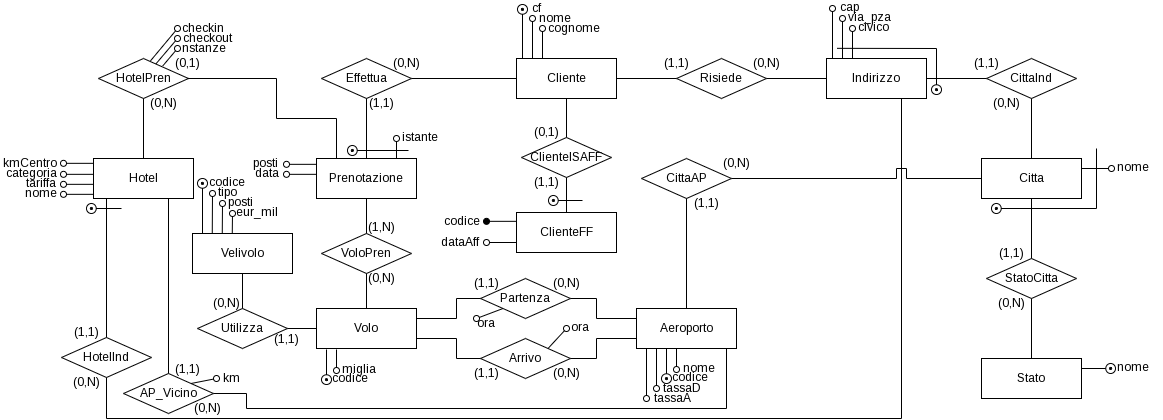
\includegraphics[width=1\textwidth]{er_ristr.png}

    \chapter{Transizione dei tipi di dati concettuali in tipi standard SQL}
      Entità Cliente: \\
      \begin{tabular}{|c|c|c|}
        \hline Attributo & Tipo & Note \\
        \hline cf & cf\_t & stringa in formato CF \\
        \hline nome & varchar(30) & \\
        \hline cognome & varchar(30) & \\
        \hline
      \end{tabular} \\ \\
    Entità ClienteFF: \\
      \begin{tabular}{|c|c|c|}
        \hline Attributo & Tipo & Note \\
        \hline codice & int\_pos & \\
        \hline dataAff & date & \\
        \hline
      \end{tabular} \\ \\
      Entità Volo: \\
      \begin{tabular}{|c|c|c|}
        \hline Attributo & Tipo & Note \\
        \hline codice & iata\_fl & \\
        \hline miglia & int\_pos & \\
        \hline
      \end{tabular} \\
      V.Volo.part\_arr: $\forall v, p, a, o_p, o_a \; $Volo$(v) \wedge $Partenza$(v, p) \wedge ora(v, p, o_p) \wedge $Arrivo$(v, a) \wedge ora(v, a, o_a) \\
      \hspace*{1cm}\rightarrow\; p \neq a$ \\
      V.Volo.no\_overbooking: $\forall v, d \; $Volo$(v) \wedge $date$(d) \;\rightarrow\; $Posti\_Voli.Posti\_Disponibili$(v, d) \geq 0$ \\ \\
      Entità Prenotazione: \\
      \begin{tabular}{|c|c|c|}
        \hline Attributo & Tipo & Note \\
        \hline istante & datetime & \\
        \hline posti & int\_pos & \\
        \hline data & date & \\
        \hline
      \end{tabular} \\ \\
      Entità Aeroporto: \\
      \begin{tabular}{|c|c|c|}
        \hline Attributo & Tipo & Note \\
        \hline codice & iata\_ap & \\
        \hline nome & varchar(50) & \\
        \hline tassaD & money\_pos & \\
        \hline tassaA & money\_pos & \\
        \hline
      \end{tabular} \\ \\
      Entità Velivolo: \\
      \begin{tabular}{|c|c|c|}
        \hline Attributo & Tipo & Note \\
        \hline codice & plane\_reg & \\
        \hline tipo & varchar(50) & \\
        \hline eur\_mil & money\_pos & \\
        \hline posti & int\_pos & \\
        \hline
      \end{tabular} \\ \\

      \newpage

      \hspace*{-0.75cm}
      Entità Hotel: \\
      \begin{tabular}{|c|c|c|}
        \hline Attributo & Tipo & Note \\
        \hline nome & varchar(50) & \\
        \hline categoria & cat\_t & \\
        \hline tariffa & money\_pos & \\
        \hline kmCentro & int\_nonneg & \\
        \hline
      \end{tabular} \\ \\
      Entità Indirizzo: \\
      \begin{tabular}{|c|c|c|}
        \hline Attributo & Tipo & Note \\
        \hline via\_pza & varchar(100) & \\
        \hline civico & int\_nonneg & 0 indica SNC \\
        \hline cap & cap\_t & \\
        \hline
      \end{tabular} \\ \\
      Entità Citta: \\
      \begin{tabular}{|c|c|c|}
        \hline Attributo & Tipo & Note \\
        \hline nome & varchar(30) & \\
        \hline
      \end{tabular} \\ \\
      Entità Stato: \\
      \begin{tabular}{|c|c|c|}
        \hline Attributo & Tipo & Note \\
        \hline nome & varchar(30) & \\
        \hline
      \end{tabular} \\ \\
      Relationship HotelPren: \\
      \begin{tabular}{|c|c|c|}
        \hline Attributo & Tipo & Note \\
        \hline checkin & date & \\
        \hline checkout & date & \\
        \hline nstanze & int\_pos & \\
        \hline
      \end{tabular} \\
      V.HotelPren.checkin\_checkout: $\forall h, p, i, o \; Hotel(h) \wedge HotelPren(h, p) \wedge \\
      \hspace*{1cm}checkin(h, p, i) \wedge checkout(h, p, o) \;\rightarrow\; i < o $ \\ \\
      Relationship AP\_Vicino: \\
      \begin{tabular}{|c|c|c|}
        \hline Attributo & Tipo & Note \\
        \hline km & int\_pos & \\
        \hline
      \end{tabular} \\ \\
      Relationship Partenza: \\
      \begin{tabular}{|c|c|c|}
        \hline Attributo & Tipo & Note \\
        \hline ora & time & \\
        \hline
      \end{tabular} \\ \\
      Relationship Arrivo: \\
      \begin{tabular}{|c|c|c|}
        \hline Attributo & Tipo & Note \\
        \hline ora & time & \\
        \hline
      \end{tabular} \\

      \section{Tipi di dati personalizzati}
        \texttt{create domain int\_pos as integer check value $>$ 0;} \\
        \texttt{create domain int\_nonneg as integer check value $\geq$ 0;} \\
        \texttt{create domain money\_pos as money check value $>$ 0;} \\
        \texttt{create domain cf\_t as char(16)} \\
        \hspace*{1cm}\texttt{check value \textasciitilde * '\textasciicircum[a-z]\{6\}[0-9]\{2\}[a-z][0-9]\{2\}[a-z][0-9]\{3\}[a-z]\$';} \\
        \texttt{create domain iata\_fl as varchar(4) check value \textasciitilde * '\textasciicircum[a-z]\{2,3\}[0-9]\{2,4\}\$';} \\
        \texttt{create domain iata\_ap as char(3) check value \textasciitilde * '\textasciicircum[a-z]\{3\}\$';} \\
        \texttt{create domain plane\_reg as varchar(5) check value \textasciitilde * '\textasciicircum[a-z]\{1,2\}\textbackslash-[a-z0-9]\{4,\}\$';} \\
        \texttt{create domain cap\_t as char(5) check value \textasciitilde * '\textasciicircum[0-9]\{5\}\$';} \\

    \chapter{Schema concettuale}
      Cliente(\underline{cf}: cf\_t, nome: varchar(30), cognome: varchar(30), via\_pza: varchar(100), \\
      \hspace*{2cm}civico: int\_nonneg, citta: varchar(30), stato: varchar(30)) \\
      \hspace*{1cm} Vincolo foreign key: (via\_pza, civico, citta, stato) references \\
      \hspace*{2cm}Indirizzo(via\_pza, civico, citta, stato) \\ \\

      \hspace*{-0.75cm}
      ClienteFF(\underline{cf}: cf\_t, codice: int\_pos, dataAff: date) \\
      \hspace*{1cm} Vincolo foreign key: cf references Cliente(cf) \\
      \hspace*{1cm} Vincolo chiave: codice \\
      \hspace*{1cm} Vincolo dominio: dataAff $\leq$ CURRENT\_DATE \\ \\

      \hspace*{-0.75cm}
      Indirizzo(\underline{via\_pza}: varchar(100), \underline{civico}: int\_nonneg, \underline{citta}: varchar(30), \underline{stato}: varchar(30), \\
      \hspace*{2cm}cap: cap\_t) \\
      \hspace*{1cm} Vincolo foreign key: (citta, stato) references Citta(nome, stato) \\ \\

      \hspace*{-0.75cm}
      Citta(\underline{nome}: varchar(30), \underline{stato}: varchar(30)) \\
      \hspace*{1cm} Vincolo foreign key: stato references Stato(nome) \\ \\

      \hspace*{-0.75cm}
      Stato(\underline{nome}: varchar(30)) \\ \\

      \hspace*{-0.75cm}
      Volo(\underline{codice}: iata\_fl, miglia: int\_pos, velivolo: plane\_reg, apPart: iata\_ap, oraPart: ora, apArr: iata\_ap, oraArr: ora) \\
      \hspace*{1cm} Vincolo foreign key: velivolo references Velivolo(codice) \\
      \hspace*{1cm} Vincolo foreign key: apPart references Aeroporto(codice) \\
      \hspace*{1cm} Vincolo foreign key: apArr references Aeroporto(codice) \\
      \hspace*{1cm} Vincolo ennupla: oraPart $<$ oraArr \\
      \hspace*{1cm} Vincolo ennupla: apPart $\neq$ apArr \\ \\

      \hspace*{-0.75cm}
      Velivolo(\underline{codice}: plane\_reg, tipo: varchar(50), eur\_mil: money\_pos, posti: int\_pos) \\ \\

      \newpage

      \hspace*{-0.75cm}
      Prenotazione(\underline{cliente}: cf\_t, \underline{istante}: datetime, posti: int\_pos, data: date) \\
      \hspace*{1cm} Vincolo foreign key: cliente references Cliente(cf) \\
      \hspace*{1cm} Vincolo inclusione: (cliente, istante) $\subseteq$ VoloPren(cpren, ipren) \\
      \hspace*{1cm} Vincolo dominio: istante $\leq$ CURRENT\_TIMESTAMP \\ \\

      \hspace*{-0.75cm}
      VoloPren(\underline{cpren}: cf\_t, \underline{ipren}: datetime, volo: iata\_fl) \\
      \hspace*{1cm} Vincolo foreign key: (cpren, ipren) references Prenotazione(cliente, istante) \\
      \hspace*{1cm} Vincolo foreign key: volo references Volo(codice) \\ \\

      \hspace*{-0.75cm}
      Aeroporto(\underline{codice}: iata\_ap, nome: varchar(50), tassaD: money\_pos, tassaA: money\_pos, \\
      \hspace*{2cm}citta: varchar(30), stato: varchar(30)) \\
      \hspace*{1cm} Vincolo foreign key: (citta, stato) references Citta(nome, stato) \\ \\

      \hspace*{-0.75cm}
      Hotel(\underline{via\_pza}: varchar(100), \underline{civico}: int\_nonneg, \underline{citta}: varchar(30), \underline{stato}: varchar(30), \\
      \hspace*{2cm}nome: varchar(50), categoria: cat\_t, tariffa: money\_pos, kmCentro: int\_nonneg) \\
      \hspace*{1cm} Vincolo foreign key: (via\_pza, civico, citta, stato) references \\
      \hspace*{2cm}Indirizzo(via\_pza, civico, citta, stato) \\
      \hspace*{1cm} Vincolo foreign key: (via\_pza, civico, citta, stato) references \\
      \hspace*{2cm}AP\_Vicino(via\_pza, civico, citta, stato) \\ \\

      \hspace*{-0.75cm}
      AP\_Vicino(\underline{via\_pza}: varchar(100), \underline{civico}: int\_nonneg, \underline{citta}: varchar(30), \underline{stato}: varchar(30), \\
      \hspace*{2cm}\underline{ap}: iata\_ap, km: int\_pos) \\
      \hspace*{1cm} Vincolo foreign key: (via\_pza, civico, citta, stato) references \\
      \hspace*{2cm}Hotel(via\_pza, civico, citta, stato) \\
      \hspace*{1cm} Vincolo foreign key: ap references Aeroporto(codice) \\ \\

      \hspace*{-0.75cm}
      HotelPren(\underline{cliente}: cf\_t, \underline{istante}: datetime, via\_pza: varchar(100), civico: int\_nonneg, \\
      \hspace*{2cm}citta: varchar(30), stato: varchar(30), checkIn: date, checkOut: date, \\
      \hspace*{2cm}nstanze: int\_pos) \\
      \hspace*{1cm} Vincolo foreign key: (via\_pza, civico, citta, stato) references \\
      \hspace*{2cm}Hotel(via\_pza, civico, citta, stato) \\
      \hspace*{1cm} Vincolo chiave: (via\_pza, civico, citta, stato) \\
      \hspace*{1cm} Vincolo foreign key: (cliente, istante) references Prenotazione(cliente, istante) \\
      \hspace*{1cm} Vincolo ennupla: checkIn $<$ checkOut \\ \\

    \chapter{Progettazione dei vincoli esterni}
      \section{Trigger per V.Volo.no\_overbooking}
        \begin{itemize}
          \item Operazioni:
            \begin{itemize}
              \item inserimento, modifica in VoloPren
              \item modifica in Volo
              \item modifica in Velivolo
            \end{itemize}
          \item Istante di invocazione: prima dell'operazione intercettata
          \item Funzione:
            \begin{enumerate}[label*=\arabic*.]
              \item Sia error = FALSE;
              \item Sia new l'ennupla che si sta inserendo oppure il risultato della modifica;
              \item Sia old il valore dell'ennupla prima della modifica;
              \item Se l'operazione ha agito su VoloPren:
                \begin{enumerate}[label*=\arabic*.]
                  \item d := select data from Prenotazione where (cliente, istante) = (new.cpren, new.ipren);
                  \item error := check (Posti\_Voli.Posti\_Disponibili(new.volo, d) - new.posti) $<$ 0;
                \end{enumerate}
              \item Se l'operazione ha agito su Volo:
                \begin{enumerate}[label*=\arabic*.]
                  \item Se new.velivolo $\neq$ old.velivolo:
                    \begin{enumerate}[label*=\arabic*.]
                      \item pOld := select posti from Velivolo where codice = old.velivolo;
                      \item pNew := select posti from Velivolo where codice = new.velivolo;
                      \item Se pNew $<$ pOld:
                        \begin{enumerate}[label*=\arabic*.]
                          \item N := sum(select p.posti from VoloPren vp, Prenotazione p where (vp.cpren, vp.ipren) = (p.cliente, p.istante) and vp.volo = old.codice);
                          \item error := check N $>$ pNew;
                        \end{enumerate}
                    \end{enumerate}
                \end{enumerate}
              \item Se l'operazione ha agito su Velivolo:
                \begin{enumerate}[label*=\arabic*.]
                  \item Se new.posti $<$ old.posti:
                        \begin{enumerate}[label*=\arabic*.]
                          \item N := sum(select p.posti from Volo v, VoloPren vp, Prenotazione p \\
                            \hspace*{1cm}where vp.volo = v.codice and (vp.cpren, vp.ipren) = (p.cliente, p.istante) \\
                            \hspace*{1cm}and v.velivolo = old.codice);
                          \item error := check N $>$ new.posti;
                        \end{enumerate}
                \end{enumerate}
              \item Se error = TRUE blocca l'operazione;
              \item Altrimenti permetti l'operazione;
            \end{enumerate}
        \end{itemize}

    \chapter{Specifiche realizzative degli use-case}

      \section{Registrazione}
        Registra(cf: cf\_t, nome: varchar(30), cognome: varchar(30), via\_pza: varchar(100), \\
        \hspace*{2cm}civico: int\_nonneg, citta: varchar(30), stato: varchar(30), cap: cap\_t) : cf\_t \\
        \hspace*{1cm}algoritmo:
        \texttt{
          \begin{enumerate}[label*=\arabic*]
            \item Q $\leftarrow$ risultato della query SQL ottenuta sostituendo a :cf \\
              \hspace*{1cm} il valore dell'omonimo parametro attuale \\
              \hspace*{1cm} select exists (select 1 from Cliente where cf = :cf);
            \item if Q rappresenta un errore then
            \item \hspace*{1cm} inoltra l'errore;
            \item else if Q = TRUE then
            \item \hspace*{1cm} inoltra l'errore 'cliente già esistente';
            \item else
            \item \hspace*{1cm} A $\leftarrow$ risultato della query SQL ottenuta sostituendo :via\_pza, :civico, \\
              \hspace*{2cm} :citta, :stato, :cap il valore degli omonimi parametri attuali \\
              \hspace*{2cm} select exists (select 1 from Indirizzo where (via\_pza, civico, citta, \\
              \hspace*{3cm} stato, cap) = (:via\_pza, :civico, :citta, :stato, :cap);
            \item \hspace*{1cm} if A rappresenta un errore then
            \item \hspace*{2cm} inoltra l'errore;
            \item \hspace*{1cm} else if A = FALSE then
            \item \hspace*{2cm} IAddr $\leftarrow$ risultato della query SQL ottenuta sostituendo :via\_pza, \\
              \hspace*{3cm} :civico, :citta, :stato, :cap il valore degli omonimi \\
              \hspace*{3cm} parametri attuali \\
              \hspace*{3cm} insert into Indirizzo values (:via\_pza, :civico, :citta, \\
              \hspace*{4cm} :stato, :cap);
            \item \hspace*{2cm} if IAddr rappresenta un errore then
            \item \hspace*{3cm} inoltra l'errore;
            \item \hspace*{1cm} ICl $\leftarrow$ risultato della query SQL ottenuta sostituendo a :cf, \\
              \hspace*{2cm} :nome, :cognome, :via\_pza, :civico, :citta, :stato il valore \\
              \hspace*{2cm} degli omonimi parametri attuali \\
              \hspace*{2cm} insert into Clienti values (:cf, :nome, :cognome, :via\_pza, \\
              \hspace*{3cm} :civico, :citta, :stato);
            \item \hspace*{1cm} if ICl rappresenta un errore then
            \item \hspace*{2cm} inoltra l'errore;
            \item \hspace*{1cm} else return :cf;
          \end{enumerate}
        }

      \section{Prenotazione\_Voli}
        Prenota(cliente: cf\_t, v: iata\_fl, nposti: int\_pos, giorno: date) : (cf\_t, datetime) \\
        \hspace*{1cm}algoritmo:
        \begin{enumerate}[label*=\arabic*]
          \item \texttt{disp $\leftarrow$ Posti\_Voli.Posti\_Disponibili(v, giorno);}
          \item \texttt{if nposti $>$ disp then}
          \item \texttt{\hspace*{1cm} inoltra l'errore 'posti non disponibili';}
          \item \texttt{else}
          \item \texttt{\hspace*{1cm} ist $\leftarrow$ CURRENT\_TIMESTAMP;}
          \item \texttt{\hspace*{1cm} I $\leftarrow$ risultato della transazione SQL ottenuta sostituendo :cliente, :posti, \\
            \hspace*{2cm} :giorno, :volo con gli omonimi parametri attuali \\
            \hspace*{2cm} begin transaction; \\
            \hspace*{2cm} insert into Prenotazione values(:cliente, ist, :posti, :giorno); \\
            \hspace*{2cm} insert into VoloPren values(:cliente, ist, :volo); \\
            \hspace*{2cm} commit work;}
          \item \texttt{\hspace*{1cm} if I rappresenta un errore then}
          \item \texttt{\hspace*{2cm} inoltra l'errore;}
          \item \texttt{\hspace*{1cm} else return (:cliente, ist);}
        \end{enumerate}

        Annulla\_Pren(cliente: cf\_t, ist: datetime) \\
        \hspace*{1cm}algoritmo:
        \begin{enumerate}[label*=\arabic*]
          \item \texttt{Q $\leftarrow$ risultato della query SQL ottenuta sostituendo :cliente, :ist, \\
            \hspace*{2cm} con gli omonimi parametri attuali \\
            \hspace*{2cm} select exists(select 1 from Prenotazione where (cliente, istante) = (:cliente, :ist);}
          \item \texttt{if Q rappresenta un errore then}
          \item \texttt{\hspace*{1cm} inoltra l'errore;}
          \item \texttt{else if Q = FALSE then}
          \item \texttt{\hspace*{1cm} inoltra l'errore 'prenotazione non trovata';}
          \item \texttt{else}
          \item \texttt{\hspace*{1cm} D $\leftarrow$ risultato della transazione SQL ottenuta sostituendo :cliente, :ist, \\
            \hspace*{2cm} con gli omonimi parametri attuali \\
            \hspace*{2cm} begin transaction; \\
            \hspace*{2cm} delete from VoloPren where (cpren, ipren) = (:cliente, :ist); \\
            \hspace*{2cm} delete from Prenotazione where (cliente, istante) = (:cliente, :ist); \\
            \hspace*{2cm} commit work;}
          \item \texttt{\hspace*{1cm} if D rappresenta un errore then}
          \item \texttt{\hspace*{2cm} inoltra l'errore;}
          \item \texttt{\hspace*{1cm} else return;}
        \end{enumerate}

      \section{Frequent\_Flyers}
        Affilia(c: cf\_t, cod: int\_pos) : cf\_t \\
        \hspace*{1cm}algoritmo:
        \begin{enumerate}[label*=\arabic*]
          \item \texttt{Q $\leftarrow$ risultato della query SQL ottenuta sostituendo a :cf \\
            \hspace*{1cm} il valore dell'omonimo parametro attuale \\
            \hspace*{1cm} select exists (select 1 from Cliente where cf = :cf);}
          \item \texttt{if Q rappresenta un errore then}
          \item \texttt{\hspace*{1cm} inoltra l'errore;}
          \item \texttt{else if Q = FALSE then}
          \item \texttt{\hspace*{1cm} inoltra l'errore 'cliente insesistente';}
          \item \texttt{else}
          \item \texttt{\hspace*{1cm} I $\leftarrow$ risultato della query SQL ottenuta sostituendo a :cf, :cod \\
            \hspace*{2cm} i valori degli omonimi parametri attuali \\
            \hspace*{2cm} insert into ClienteFF values (:cf, :cod, CURRENT\_DATE);}
          \item \texttt{\hspace*{1cm} if I rappresenta un errore then}
          \item \texttt{\hspace*{2cm} inoltra l'errore;}
          \item \texttt{\hspace*{1cm} else return :cf;}
        \end{enumerate}

        Miglia(cf: cf\_t) : int\_pos \\
        \hspace*{1cm}algoritmo:
        \begin{enumerate}[label*=\arabic*]
          \item \texttt{Q $\leftarrow$ risultato della query SQL ottenuta sostituendo a :cf \\
            \hspace*{1cm} il valore dell'omonimo parametro attuale \\
            \hspace*{1cm} select exists (select 1 from ClienteFF where cf = :cf);}
          \item \texttt{if Q rappresenta un errore then}
          \item \texttt{\hspace*{1cm} inoltra l'errore;}
          \item \texttt{else if Q = FALSE then}
          \item \texttt{\hspace*{1cm} inoltra l'errore 'cliente insesistente o non affiliato';}
          \item \texttt{else}
          \item \texttt{\hspace*{1cm} Vnh $\leftarrow$ risultato della query SQL ottenuta sostituendo a :cf \\
            \hspace*{2cm} il valore dell'omonimo parametro attuale \\
            \hspace*{2cm} select sum(v.miglia*p.posti) from Volo v, VoloPren vp, Prenotazione p \\
            \hspace*{3cm} where v.codice = vp.volo \\
            \hspace*{3cm} and (vp.cpren, vp.ipren) = (p.cliente, p.istante) \\
            \hspace*{3cm} and p.cliente = :cf and (p.cliente, p.istante) not in \\
            \hspace*{4cm} (select cpren, ipren from HotelPren);}
          \item \texttt{\hspace*{1cm} if Vnh rappresenta un errore then}
          \item \texttt{\hspace*{2cm} inoltra l'errore;}
          \item \texttt{\hspace*{1cm} else}
          \item \texttt{\hspace*{2cm} Vh4 $\leftarrow$ risultato della query SQL ottenuta sostituendo a :cf \\
            \hspace*{3cm} il valore dell'omonimo parametro attuale \\
            \hspace*{3cm} select sum(v.miglia*p.posti) from Volo v, VoloPren vp, \\
            \hspace*{4cm} Prenotazione p, HotelPren hp, Hotel h where v.codice = vp.volo \\
            \hspace*{4cm} and (vp.cpren, vp.ipren) = (p.cliente, p.istante) \\
            \hspace*{4cm} and (hp.cpren, hp.ipren) = (p.cliente, p.istante) \\
            \hspace*{4cm} (hp.via\_pza, hp.civico, hp.citta, hp.stato) = \\
            \hspace*{5cm} (h.via\_pza, h.civico, h.citta, h.stato) \\
            \hspace*{4cm} and p.cliente = :cf and h.categoria $<$ 5;}
          \item \texttt{\hspace*{2cm} if Vh4 rappresenta un errore then}
          \item \texttt{\hspace*{3cm} inoltra l'errore;}
          \item \texttt{\hspace*{2cm} else}
          \item \texttt{\hspace*{3cm} Vh5 $\leftarrow$ risultato della query SQL ottenuta sostituendo a :cf \\
            \hspace*{4cm} il valore dell'omonimo parametro attuale \\
            \hspace*{4cm} select sum(v.miglia*p.posti) from Volo v, VoloPren vp, \\
            \hspace*{5cm} Prenotazione p, HotelPren hp, Hotel h \\
            \hspace*{5cm} where v.codice = vp.volo \\
            \hspace*{5cm} and (vp.cpren, vp.ipren) = (p.cliente, p.istante) \\
            \hspace*{5cm} and (hp.cpren, hp.ipren) = (p.cliente, p.istante) \\
            \hspace*{5cm} (hp.via\_pza, hp.civico, hp.citta, hp.stato) = \\
            \hspace*{6cm} (h.via\_pza, h.civico, h.citta, h.stato) \\
            \hspace*{5cm} and p.cliente = :cf and h.categoria = 5;}
          \item \texttt{\hspace*{3cm} if Vh5 rappresenta un errore then}
          \item \texttt{\hspace*{4cm} inoltra l'errore;}
          \item \texttt{\hspace*{3cm} else return Vnh + 2*Vh4 + 3*Vh5;}
        \end{enumerate}

      \section{Posti\_Voli}
        Posti\_Disponibili(v: iata\_fl, d: date) : int\_nonneg \\
        \hspace*{1cm}algoritmo:
        \begin{enumerate}[label*=\arabic*]
          \item \texttt{N $\leftarrow$ risultato della query SQL ottenuta sostituendo a :v e :d \\
            \hspace*{1cm} i valori degli omonimi parametri attuali \\
            \hspace*{1cm} select a.posti as maxp sum(p.posti) as occp from Prenotazione p, \\
            \hspace*{1cm} VoloPren vp, Volo v, Velivolo a \\
            \hspace*{1cm} where (p.cliente, p.istante) = (vp.cpren, vp.ipren) and vp.volo = volo.codice \\
            \hspace*{1cm} and volo.codice and volo.velivolo = a.codice and v.codice = :v \\
            \hspace*{1cm} and p.data = :d group by (a.posti);}
          \item \texttt{if N rappresenta un errore then}
          \item \texttt{\hspace*{1cm} inoltra l'errore;}
          \item \texttt{else return N.maxp - N.occp;}
        \end{enumerate}

      \section{Costo\_Biglietti}
        Costo(v: iata\_fl, d: date) : money\_pos \\
        \hspace*{1cm}algoritmo:
        \begin{enumerate}[label*=\arabic*]
          \item \texttt{N $\leftarrow$ risultato della query SQL ottenuta sostituendo a :v e :d \\
            \hspace*{1cm} i valori degli omonimi parametri attuali \\
            \hspace*{1cm} select apD.tassaD, apA.tassaA, v.miglia, v.eur\_mil, a.posti \\
            \hspace*{1cm} from Aeroporto apD, Aeroporto apA, Volo v, Velivolo a \\
            \hspace*{1cm} where apD.codice = v.apPart and apA.codice = v.apArr \\
            \hspace*{1cm} and v.velivolo = a.codice;}
          \item \texttt{if N rappresenta un errore then}
          \item \texttt{\hspace*{1cm} inoltra l'errore;}
          \item \texttt{else}
          \item \texttt{\hspace*{1cm} base $\leftarrow$ (N.miglia*N.eur\_mil + N.tassaD + N.tassaA)/N.posti * 1.2;}
          \item \texttt{\hspace*{1cm} disp $\leftarrow$ Posti\_Voli.Posti\_Disponibili(:v, :d);}
          \item \texttt{\hspace*{1cm} disp\_coeff $\leftarrow$ (disp $\geq$ N.posti/2) ? 0.8 * disp : 1.2 * disp;}
          \item \texttt{\hspace*{1cm} return base * disp\_coeff;}
        \end{enumerate}

      \newpage

      \section{Consiglia\_Hotel}
        Consiglia\_Hotel(c: varchar(30), s: varchar(30), maxt: money\_pos) : \\
        \hspace*{2cm}(varchar(100), int\_nonneg, varchar(30), varchar(30))(1,N) \\
        \hspace*{1cm}algoritmo: \\
        \begin{enumerate}[label*=\arabic*]
          \item \texttt{H $\leftarrow$ risultato della query SQL ottenuta sostituendo a :c, :s, :maxt \\
            \hspace*{1cm} i valori degli omonimi parametri attuali \\
            \hspace*{1cm} select via\_pza, civico, citta, stato, categoria, kmCentro from Hotel \\
            \hspace*{1cm} where (citta, stato) = (:c, :s) and tariffa $\leq$ :maxt \\
            \hspace*{1cm} order by kmCentro asc;}
          \item \texttt{if H rappresenta un errore then}
          \item \texttt{\hspace*{1cm} inoltra l'errore;}
          \item \texttt{else}
          \item \texttt{\hspace*{1cm} cons $\leftarrow$ \{H[0]\};}
          \item \texttt{\hspace*{1cm} for i $\leftarrow$ 1 to length(H-1) do}
          \item \texttt{\hspace*{2cm} if (H[i].categoria = H[0].categoria}
          \item \texttt{\hspace*{4cm} and H[i].kmCentro $\leq$ H[0].kmCentro*1.1)}
          \item \texttt{\hspace*{4cm} or (H[i].categoria $>$ H[0].categoria}
          \item \texttt{\hspace*{4cm} and H[i].kmCentro $\leq$ H[0].kmCentro*1.2) then}
          \item \texttt{\hspace*{3cm} cons $\leftarrow$ append(cons, H[i]);}
          \item \texttt{\hspace*{1cm} done;}
          \item \texttt{\hspace*{1cm} return cons;}
        \end{enumerate}

\end{document}
